\documentclass[11pt]{article}

% load some asm stuff -
\usepackage{amssymb}
\usepackage{amsmath}
\usepackage{amsthm}
%\usepackage{palatino,lettrine}
\usepackage{fancyhdr}
\usepackage{epsfig}
\usepackage[square,sort,comma,numbers]{natbib}
\usepackage{simplemargins}
\usepackage{setspace}
\usepackage{wrapfig}
\usepackage{hyperref}
%\usepackage{boiboites}
\usepackage[margin=0pt,font=small,labelfont=bf]{caption}
\newcommand{\boldindex}[1]{\textbf{\hyperpage{#1}}}
\usepackage{makeidx}\makeindex
\bibliographystyle{plos2015}

\usepackage{algpseudocode}
\usepackage{algorithm}


% Set the size
%\textwidth = 6.75 in
%\textheight = 9.75 in
%\oddsidemargin = 0.0 in
%\evensidemargin = 0.0 in
%\topmargin = 0.01 in
%\headheight = 0.0 in
%\headsep = 0.25 in
%\parskip = 0.15in
% \doublespace
\setallmargins{1in}

\newtheorem{example}{Example}[section]
\newtheorem{thm}{Theorem}[section]
\newtheorem{property}{Property}[section]

\theoremstyle{definition}
\newtheorem{defn}[thm]{Definition}

\makeatletter
% \renewcommand\subsection{\@startsection
% 	{subsection}{2}{0mm}
% 	{-0.05in}
% 	{0.05\baselineskip}
% 	{\normalfont\normalsize\bfseries}}
\renewcommand\subsubsection{\@startsection
	{subsubsection}{2}{0mm}
	{-0.05in}
	{-0.5\baselineskip}
	{\normalfont\normalsize\itshape\bfseries}}
\renewcommand\paragraph{\@startsection
	{paragraph}{2}{0mm}
	{-0.05in}
	{-0.5\baselineskip}
	{\normalfont\normalsize\itshape}}
\makeatother
\linespread{1.1}

\fancypagestyle{proposal}{\fancyhf{}%
	\fancyhead[RO,LE]{\thepage}%
	\fancyhead[LO,RE]{CHEME 133 Module 1 European Options Contracts}%
	\renewcommand\headrulewidth{1pt}}
\pagestyle{proposal}

\usepackage{mdframed}
\definecolor{lgray}{rgb}{0.92,0.92,0.92}
\definecolor{antiquewhite}{rgb}{0.98,0.92,0.84}
\definecolor{lightskyblue}{rgb}{0.93,0.95,0.99}

% defn environment
\mdfdefinestyle{theoremstyle}{% 
    linecolor=black,linewidth=1pt,% 
    frametitlerule=true,% 
    frametitlebackgroundcolor=lgray, 
    innertopmargin=\topskip,} 
\mdtheorem[style=theoremstyle]{definition}{Definition}

% concept environment
\mdfdefinestyle{conceptstyle}{% 
    linecolor=black,linewidth=1pt,% 
    frametitlerule=true,% 
    frametitlebackgroundcolor=lightskyblue, 
    innertopmargin=\topskip,} 
\mdtheorem[style=conceptstyle]{concept}{Concept}
\newcommand{\newterm}[1]{{\it #1}}

% Single space'd bib -
\setlength\bibsep{0pt}

\renewcommand{\rmdefault}{phv}\renewcommand{\sfdefault}{phv}
%\newboxedtheorem[boxcolor=black, background=gray!5,titlebackground=orange!20,titleboxcolor = black]{color_box_example}{Example}{test}

% Change the number format in the ref list -
\renewcommand{\bibnumfmt}[1]{#1.}

% Change Figure to Fig.
\renewcommand{\figurename}{Fig.}
\usepackage{enumitem}
\setlist{noitemsep} % or \setlist{noitemsep} to leave space around whole list

%Joycelyn Chan, Joshua Lequieu, Michael Paull, Chidanand Balaji, Ryan Tasseff
%Our derivation follows closely the earlier development of Fredrickson \citep{Fredrickson:1976fk}.

% Begin ...
\begin{document}

%\begin{titlepage}
{\par\centering\textbf{\Large CHEME 133 Module 1: Introduction to Derivatives and European Style Options Contracts at Expiration}}
\vspace{0.2in}
{\par \centering \large{Jeffrey D. Varner}}
\vspace{0.05in}
{\par \centering \large{Smith School of Chemical and Biomolecular Engineering}}
{\par \centering \large{Cornell University, Ithaca NY 14853}}
% \vspace{0.1in}
% {\par \centering \small{Copyright \copyright\ Jeffrey Varner 2018. All Rights Reserved.}}\\

%\end{titlepage}
\date{}
\thispagestyle{empty}

\setcounter{page}{1}

\section*{Introduction}
Derivatives are one of the three primary financial instrument categories: derivatives, equity (i.e., shares of stock), and debt (i.e., bonds and mortgages). 
Derivatives provide payoffs that depend on the value of other assets, such as commodities, bonds, stocks, or market indexes. 
Thus, the value of a derivative is based mainly on the price movements of an underlying asset, e.g., stocks, commodities, currencies, etc. 
This course will focus exclusively on options, a derivative product that uses stock as its underlying asset. 
Like bonds, options are contractural agreements between buyers and sellers to conduct a particular transaction at some later date. 
Options, derivatives that use equity, i.e., shares of a stock or an exchange-traded fund, as their underlying asset, 
are structured agreements between a buyer and a seller that give the option buyer the right, but not the obligation, 
to execute the transaction described in the contract, i.e., to buy (or sell) an underlying asset in some predetermined way in a specified time frame. 
The predetermined price is the strike price, and the specified period is the contract's lifetime, where the lifetime ends on the expiration date. 

Investors can use options and other derivatives to \href{https://www.investopedia.com/terms/h/hedge.asp}{hedge} against future asset price movements or for speculation. 
For example, a trader can buy an option contract instead of shares of an underlying stock to generate profits from the underlying stock's price movements, 
typically at a lower cost than the corresponding block of shares. Options contracts are traded on exchanges throughout the world; 
the \href{https://www.cboe.com}{The Chicago Board Options Exchange} is the largest options exchange in the United States, 
responsible for approximately 33\% of the daily options trading volume in the United States (about 32 million contracts are traded each day in the United States in 2023). 
Worldwide, in 2023, there were \href{https://www.fia.org/fia/articles/global-futures-and-options-volume-hits-record-137-billion-contracts-2023}{approximately 137 billion derivatives contracts traded annually}.
Options are also attractive because they offer \href{https://www.merrilledge.com/investment-products/options/options-trading-leverage-risk}{leverage}, 
i.e., an option contract can control a unit of asset, e.g., 100 shares of a stock, 
at a cost that is typically less than the market value of that asset. 
This allows option buyers to pay a relatively small premium for market exposure in relation to the value of the underlying asset. 
An option buyer can see significant gains from comparatively small percentage moves in the underlying asset's price. 
However, leverage also has a considerable downside. 
For example, if the underlying asset price does not rise or fall as anticipated during the lifetime of the option contract, 
leverage magnifies the investment's percentage loss.

In this module, we'll begin our study of derivatives, and options in particular, by focusing on European-style options contracts.
For European-style contracts, holders can only exercise their right on the expiration date.
However, for American-style contracts, which we'll consider later, the holder can exercise their right on or before the expiration date.
We'll study the two types of options contracts: \texttt{call} contracts and \texttt{put} contracts (Fig. \ref{fig:options-schematic}).

% The holder of the option pays a premium for the right to buy or sell the underlying asset. 
% The premium is the price of the option.

\begin{figure}[ht]
    \centering
    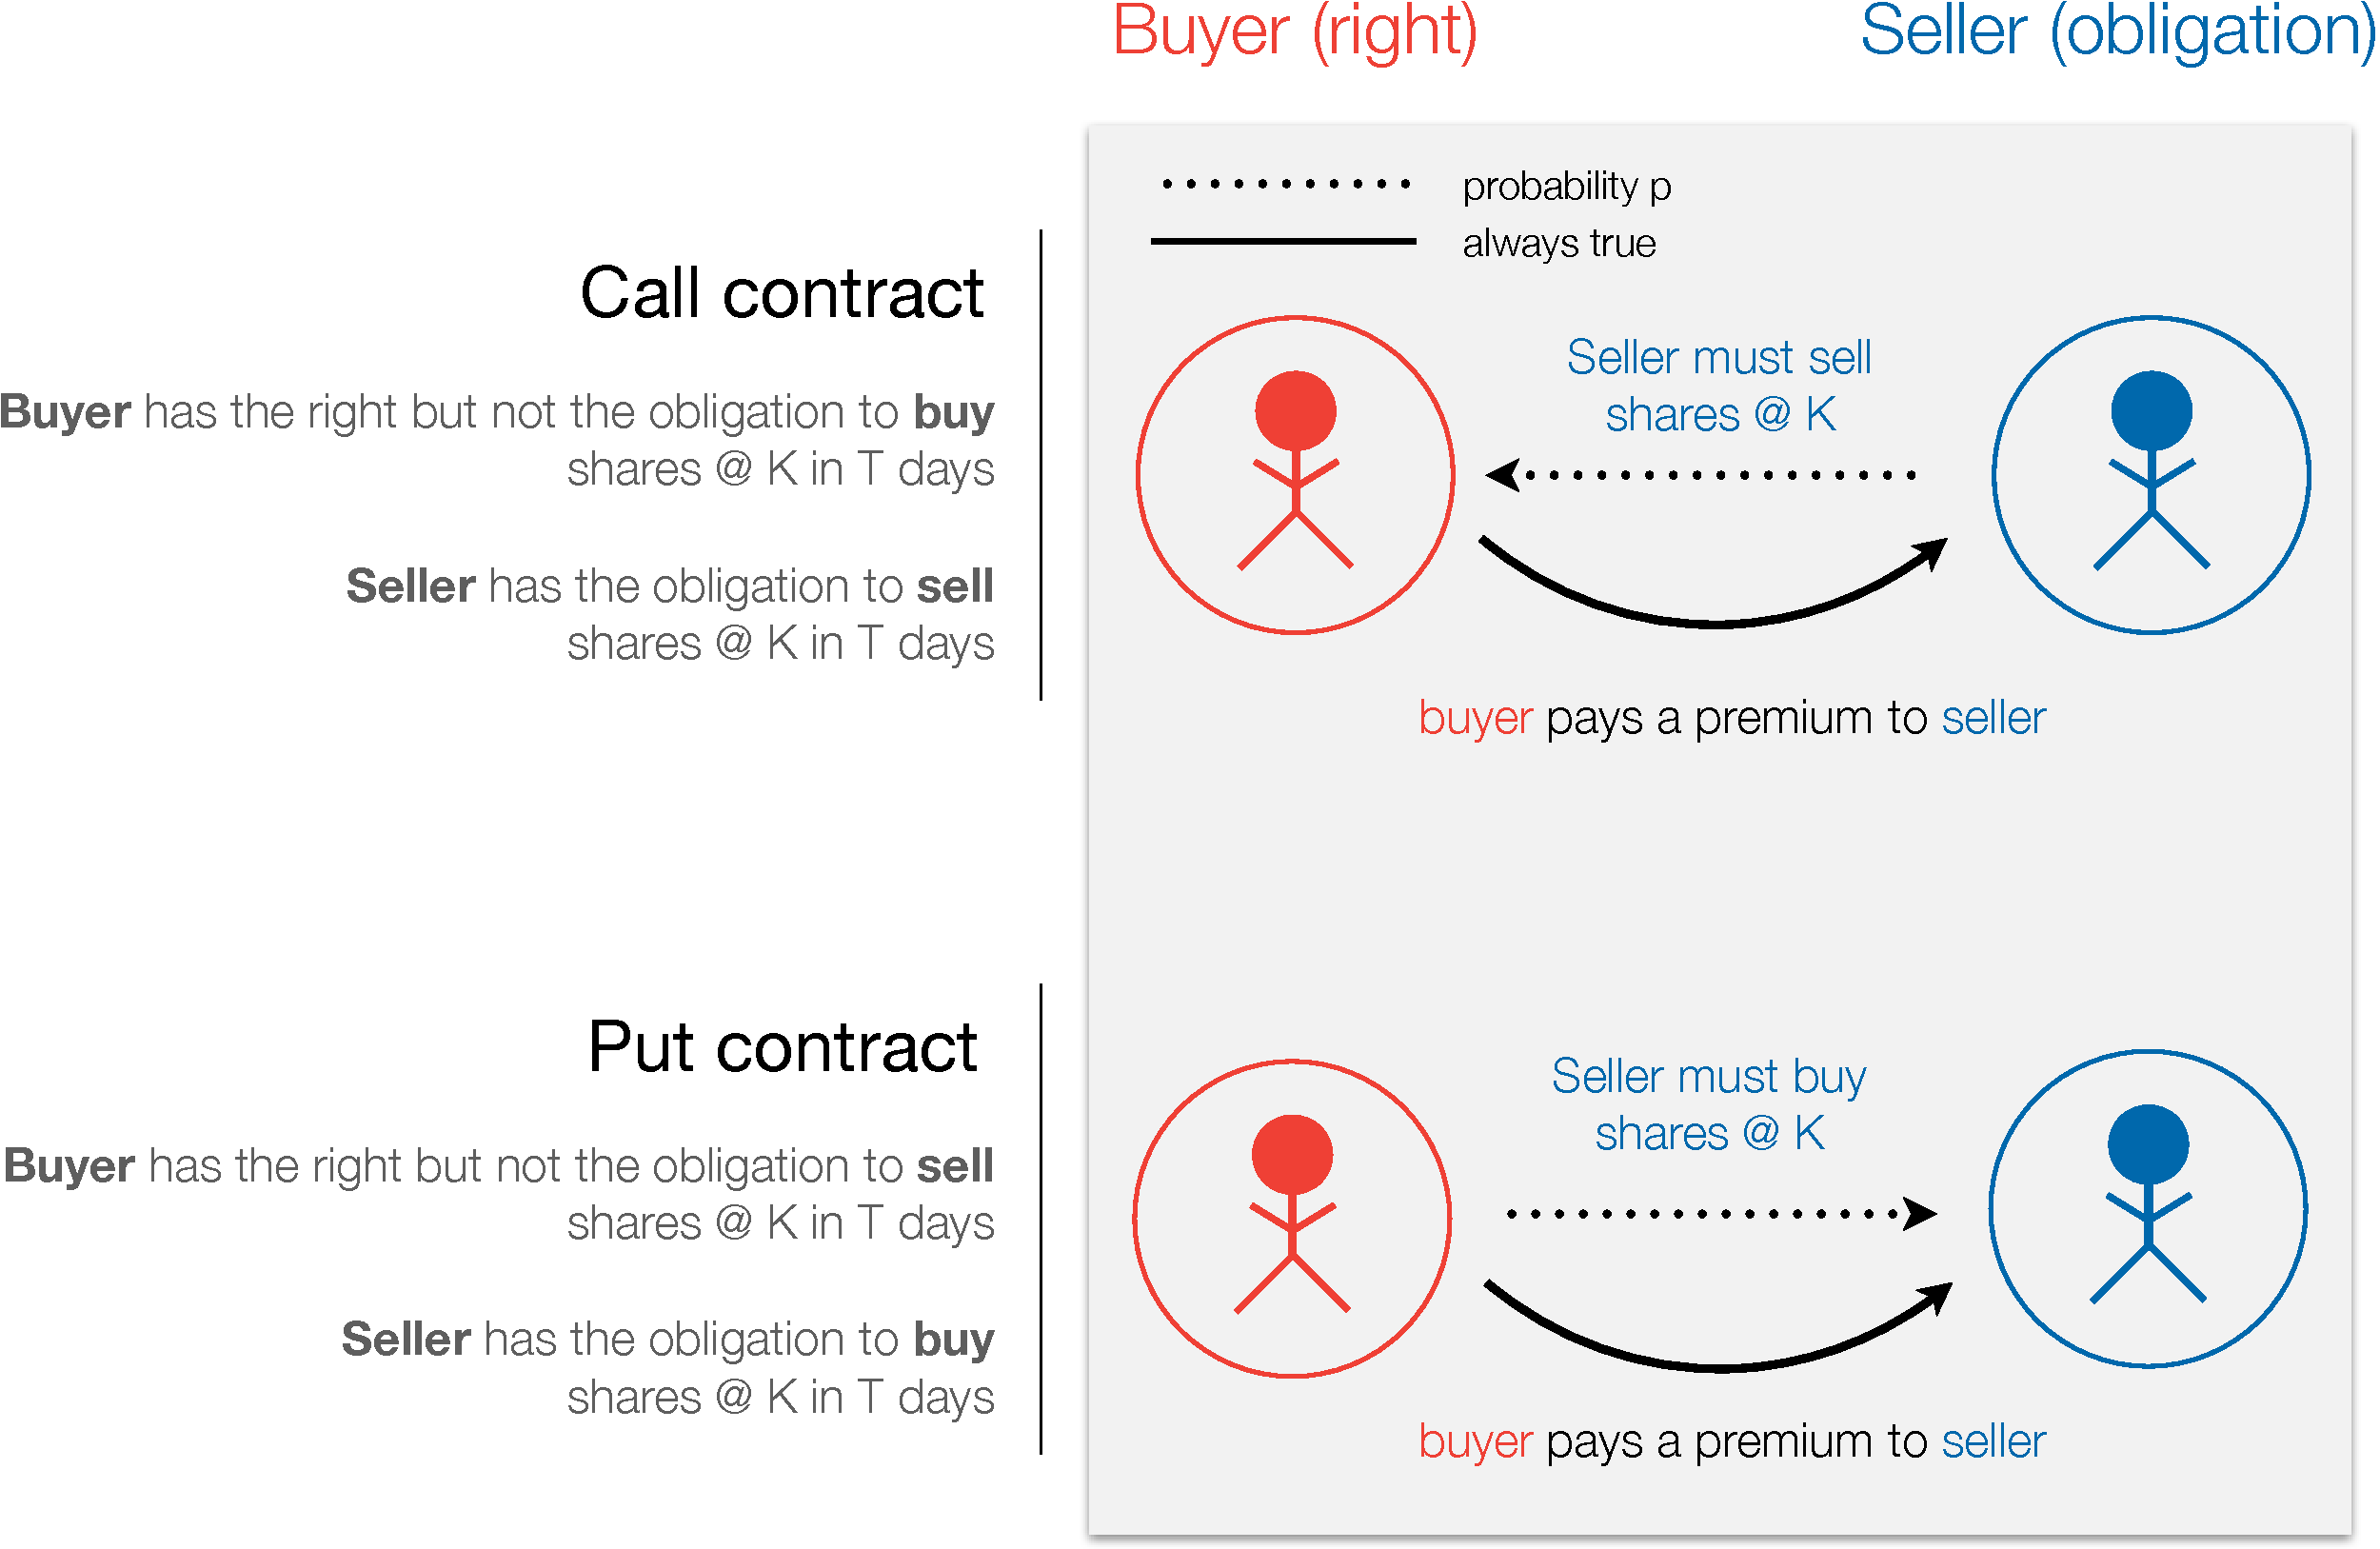
\includegraphics[width=0.85\textwidth]{./figs/Fig-Options-Table-Schematic.pdf}
    \caption{Schematic of call and put options contracts. The buyer pays a premium to the seller for the right, but 
	not the obligation to transact in the future, where the contract describes the transaction parameters.}\label{fig:options-schematic}
\end{figure}

\subsection*{Call and Put Contracts}
A \texttt{call} contract gives the holder (buyer) the right, but not the obligation, to purchase a specified asset, 
such as stocks, commodities, or currencies, to their counterparty (contract seller). 
Let's consider stock as the underlying asset. A single standard options contract controls 100 shares of stock. 
From the buyer's perspective, call contracts allow an investor to benefit from the upside price movement of a stock without purchasing the stock.
Further, call options (again from the buyer's perspective) have limited downside risk, i.e., the maximum amount the holder of the call option can lose 
is the premium paid for the option. Finally, call options are a mechanism to purchase shares of stock at the strike price of $K$ instead of the market price of $S$. 
On the other hand, from the seller's perspective, the main objective of selling a call contract is to collect the premium $\mathcal{P}$. 
Call contracts also allow the seller to benefit from downward price movement without purchasing shares of stock (in the case of a naked call).
However, for a seller, call options have unlimited upside risk; 
Thus, call options are often only sold by investors who already own the required number of shares of stock 
(known as a \href{https://www.investopedia.com/terms/c/coveredcall.asp}{covered call position}. 
Finally, call options offer the seller the opportunity to sell shares of stock at the strike price of $K$ instead of the market price of $S$.

A \texttt{put} contract gives the holder (buyer) the right, but not the obligation, to sell a specified asset, 
such as stocks, commodities, or currencies, at a specified price to their counterparty (contract seller). 
Let's consider stock as the underlying asset. A single standard put contract controls 100 shares of stock.
From the buyer's perspective, put contracts allow an investor to benefit from the downward price movement of a stock without purchasing the stock. 
Further, put options (again from the buyer's perspective) have limited downside risk, i.e., the maximum amount the put option holder can lose is the premium paid for the option. 
Finally, put contracts are a mechanism to sell shares of stock at the strike price of $K$ instead of the market price of $S$. 
From the seller's perspective, the motivation for selling a put contract is to collect the premium $\mathcal{P}$. 
Put contracts also allow the seller to benefit from the price movement to the upside without purchasing shares.
However, for a seller, put options have unlimited downside risk; 
thus, put options are often only sold by investors who have set aside the required capital to purchase the required number of shares of stock 
(known as a \href{https://www.fidelity.com/learning-center/investment-products/options/know-about-cash-covered-puts}{cash-secured put position}).
Finally, put options offer the seller the opportunity to buy shares of a firm at the strike price of $K-\mathcal{P}$ instead of the market price of $S$.

\begin{concept}[Jargon: Long and Short Contracts]\label{concept:long-short-contracts}

	\textbf{Long contracts}: Instead of saying the \texttt{call} (or \texttt{put})) contract holder or buyer, you may sometimes hear the term \texttt{long call} (or \texttt{long put}) to denote a person has purchased a \texttt{call} (or \texttt{put}) contract.
	Thus, a person who buys an options contract is said to be \texttt{long} the \texttt{call} (or \texttt{put}) contract.
	
	\vspace{0.01in}
	\noindent\textbf{Short contracts}: On the other hand, instead of saying the \texttt{call} (or \texttt{put}) contract seller, you may hear the term \texttt{short call} (or \texttt{short put}) to denote a person has sold a \texttt{call} (or \texttt{put}) contract.
	Thus, a person who sells an options contract is said to be \texttt{short} the contract.
\end{concept}

\section*{Payoff and Profit Diagrams for Long Contracts}
Unlike equity, e.g., shares of a stock or ETF, which have a linear payoff profile, both long and short options contracts have a nonlinear payoff profile depending on the price of the underlying asset at expiration, 
the strike price of the contract, the premium paid for the contract, and the type of contract (call or put).
For now, let's focus on long contracts, i.e., the buyer of the contract.

\subsection*{Call Options}
The payoff per share at expiration at time $t = T$ for a \texttt{call} option is:
\begin{equation}
V_{c}(K,S(T)) = \max\left(S(T) - K,~0\right)
\end{equation}
where $K$ denotes the strike price and $S(T)$ is the share price at expiration. 
The \texttt{seller} charges the \texttt{buyer} a premium at time $t=0$ (now), which we denote as $\mathcal{P}_{c}(K,S(0))$, for each contract.
Thus, the buyer's profit per share at expiration is the contract payoff minus the contract premium:
\begin{equation}
P_{c}(K,S(T)) = V_{c}(K,S(T)) -  \mathcal{P}_{c}(K,S(0))
\end{equation}
where $P_{c}(K,S(T)) = 0$ denotes the breakeven point for the buyer. 
Substituting the payoff and profit expressions into the breakeven equation, 
gives the breakeven share price $\mathcal{B}_{c}$ at expiration for the buyer 
of the \texttt{call} contract:
\begin{equation}
\mathcal{B}_{c} = K + \mathcal{P}_{c}(K,S(0))
\end{equation}
Thus, the share price at expiration must exceed the sum of the strike price and the premium for the buyer to make a profit.
An example payoff, profit, and breakeven diagram for a \texttt{call} contract from the buyer's perspective 
is shown in Fig. \ref{fig:call-payoff-profit-breakeven-diagram}.  
\begin{figure}[ht]
    \centering
    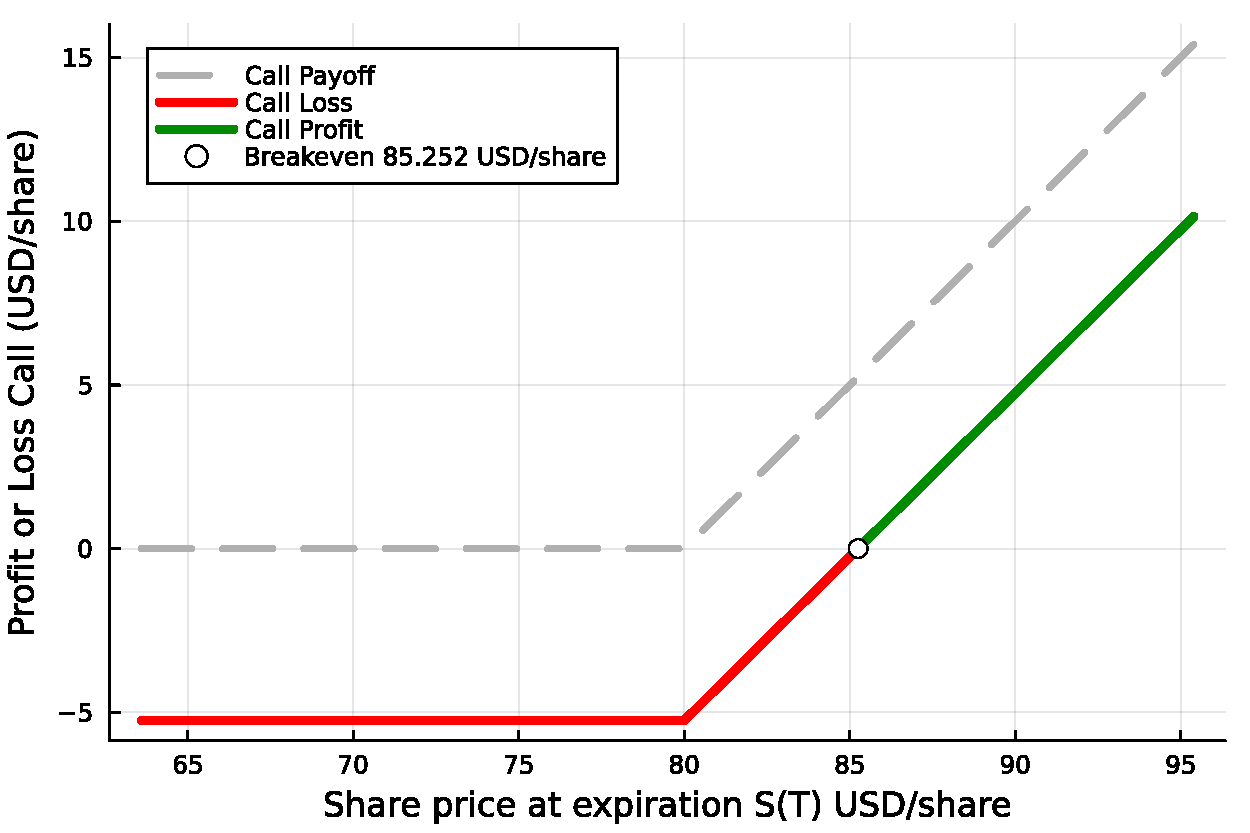
\includegraphics[width=0.65\textwidth]{./figs/Fig-Example-Call-K80-62DTE.pdf}
    \caption{Schematic of the payoff, profit and breakeven for a \texttt{long call} 
	contract. The gray dashed line denotes the payoff at expiration for the buyer.
	The red line denotes share prices at expiration that result in a loss for the buyer, 
	while the green line denotes share prices at expiration that result in a profit for the buyer.
	Parameters: the \texttt{call} 
	contract strike price is $K$ = 80 USD/share and the premium $\mathcal{P}_{c}$ = 5.25 USD/share.}\label{fig:call-payoff-profit-breakeven-diagram}
\end{figure}

% we can construct the payoff and profit diagrams for a call option (Fig. \ref{fig:call-option-payoff-profit}).
% The premium (cost) for each contract is governed by:
% \begin{equation*}
% \mathcal{P}_{c}(K,S(0))\geq\mathbb{E}\Bigl(\mathcal{D}^{-1}_{T,0}(\bar{r})\cdot{V_{c}}(K,S(T))\Bigr)
% \end{equation*}
% where $\mathcal{D}_{T,0}(\bar{r})$ denotes the risk neutral discount factor computed between purchase and contract expiration.

\subsection*{Put Options}
The payoff per share at expiration for a put option contract is given by:
\begin{equation}
V_{p}(K,S(T)) = \max\left(K - S(T),~0\right)
\end{equation}
where $K$ denotes the strike price and $S(T)$ is the share price at expiration. 
The \texttt{seller} charges the \texttt{buyer} a premium $\mathcal{P}_{p}(K,S(0))$ for each contract.
The buyer's profit per share at expiration is the payoff minus the contract premium:
\begin{equation}
P_{p}(K,S(T)) = V_{p}(K,S(T)) -  \mathcal{P}_{p}(K,S(0))
\end{equation}
where $P_{p}(K,S(T)) = 0$ denotes the breakeven point for the buyer. 
Substituting the payoff and profit expressions into the breakeven equation gives the breakeven share price $\mathcal{B}_{p}$ at expiration for the buyer 
of the \texttt{put} contract:
\begin{equation}
\mathcal{B}_{p} = K - \mathcal{P}_{p}(K,S(0))
\end{equation}
Thus, the share price at expiration must fall below the strike price minus the premium for the buyer of the \texttt{put} 
contract to make a profit.

\begin{figure}[ht]
    \centering
    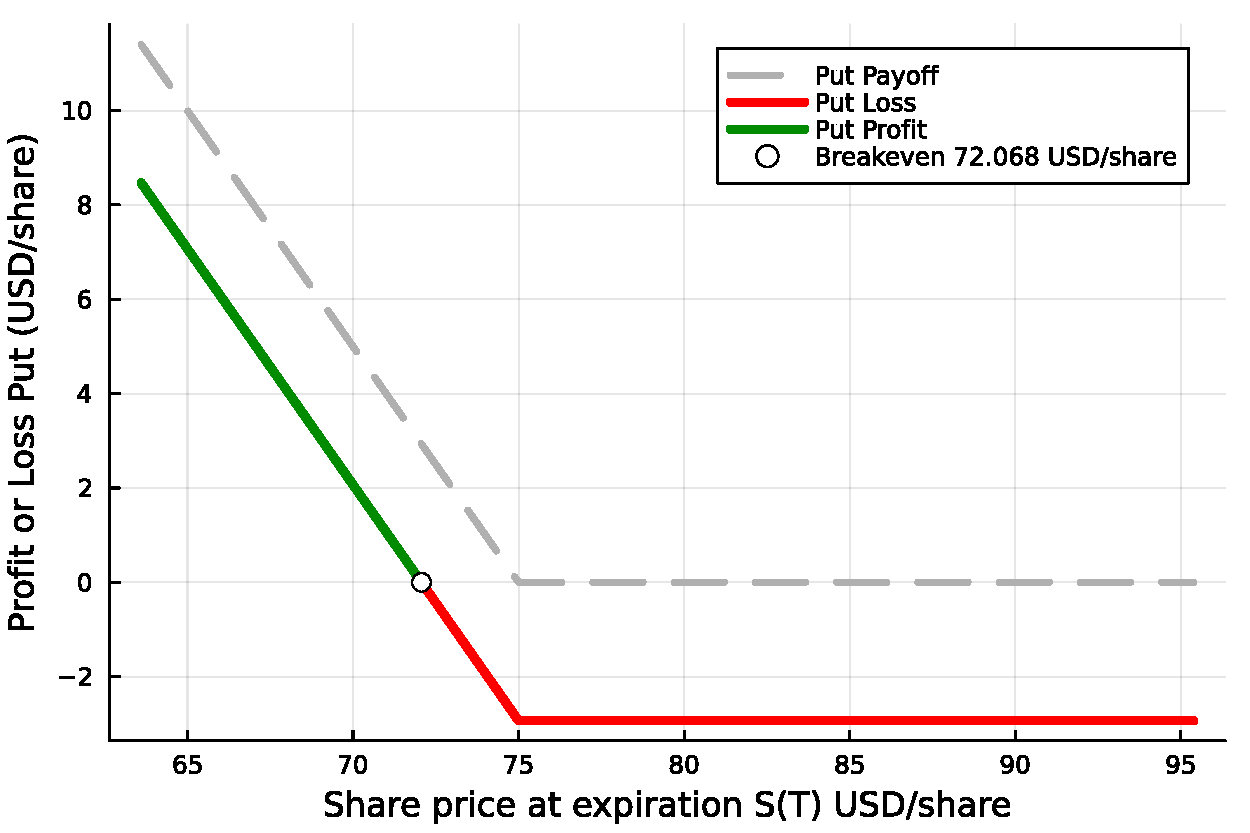
\includegraphics[width=0.65\textwidth]{./figs/Fig-Example-Put-K75-62DTE.pdf}
    \caption{Schematic of the payoff, profit and breakeven for a \texttt{long call} 
	contract. The gray dashed line denotes the payoff at expiration for the buyer.
	The red line denotes share prices at expiration that result in a loss for the buyer, 
	while the green line denotes share prices at expiration that result in a profit for the buyer.
	Parameters: the \texttt{put} 
	contract strike price is $K$ = 75 USD/share and a midpoint of premium $\mathcal{P}_{c}$ = 2.93 USD/share.}\label{fig:put-payoff-profit-breakeven-diagram}
\end{figure}

% The premium (cost) for a put contract is governed by:
% \begin{equation}
% \mathcal{P}_{p}(K,S(0))\geq\mathbb{E}\Bigl(\mathcal{D}^{-1}_{T,0}(\bar{r})\cdot{V_{p}}(K,S(T))\Bigr)
% \end{equation}
% where $\mathcal{D}_{T,0}(\bar{r})$ denotes the risk neutral discount factor computed between purchase and expiration.

\section*{European Contracts Premiums}
An option's premium is the price the buyer pays the seller for the right to buy or sell an underlying asset at a specified price.
There are many methods to compute the premium of an options contract, but the most widely used method (by far) is the Black-Scholes-Merton (BSM) model (and its extensions).
The BSM model has a closed-form solution, i.e., a mathematical expression that can be evaluated directly. Thus, it is computationally efficient.
Alternatively, the premium of an options contract can be computed using numerical methods, such as binomial trees or Monte Carlo simulation.
Let's consider the BSM model first, and then we'll explore a Monte Carlo method to price European calls and put contracts.

\subsection*{The Black-Scholes-Merton (BSM) Model}
The Black-Scholes-Merton model is used to compute the premium of European-style options contracts \cite{BlackScholes1973};
Robert C. Merton, Myron S. Scholes, and Fischer Black won the \href{https://www.nobelprize.org/prizes/economic-sciences/1997/press-release/}{Nobel Prize in Economics in 1997} for their work on this model.
The model assumes that the underlying asset's price follows a geometric Brownian motion with constant drift and volatility, where the drift is the risk-free interest rate, i.e., we evaluate the option using a risk-neutral pricing paradigm.
Further, the model assumes that the risk-free interest rate is constant and that the underlying stock does not pay dividends (although the model can be modified to include dividends).
Under these assumptions, the price of the option can be computed using the Black-Scholes-Merton pricing formula, which is the parabolic partial differential equation:
\begin{eqnarray}\label{eqn:BSM-pde}
	\frac{\partial{V}}{\partial{t}} + \frac{1}{2}\sigma^{2}S^{2}\frac{\partial^{2}V}{\partial{S}^{2}} & = & \bar{r}V - rS\frac{\partial{V}}{\partial{S}}  \\
	\frac{dS}{S} & = & \bar{r}\,dt + \sigma\,{dW}\\
	V(T,S) & = & K(S)
\end{eqnarray}
where $V(t, S)$ is the price of the option, $S$ is the price of the underlying asset (governed by the risk-neutral geometric Brownian motion model), 
$K(S)$ is the payoff of the option at expiration, $T$ is the expiration date, $t$ is time, 
$\bar{r}$ is the risk-free interest rate, and $\sigma$ is the volatility of the underlying asset.
$t$ is time, $r$ is the risk-free interest rate, and $\sigma$ is the volatility of the underlying asset.
While we could solve the partial differential equation \ref{eqn:BSM-pde} directly, it is more common to use the closed-form solution of the Black-Scholes-Merton pricing formula.

The price of a European \texttt{call} option is given by Definition \ref{defn:BSM-call-closed-form}:
\begin{definition}[Black-Scholes-Merton Pricing Formula for a European Call Option]\label{defn:BSM-call-closed-form}
The Black-Scholes-Merton pricing formula for a European \texttt{call} option is given by the expression:
\begin{equation}
	\mathcal{P}_{c}(K,S(0)) = N(d_{+})S(0) - N(d_{-})K\mathcal{D}^{-1}_{T,0}(\bar{r})
\end{equation}
where $N(\dots)$ denotes the standard normal cumulative distribution function, $S(0)$ is the price of the underlying asset at time $t=0$ (when we are evaluating the option),
$K$ is the strike price of the contract, and $\mathcal{D}^{-1}_{T,0}(\bar{r})$ is the discount factor from time $t=0$ to time $T$ evaluated at the risk-free interest rate $\bar{r}$.
The arguments of the normal cumulative distribution function are given by:
\begin{eqnarray}
d_{+} & = & \frac{1}{\sigma\sqrt{T}}\left[\ln(\frac{S_{\circ}}{K}) + (\bar{r}+\frac{\sigma^{2}}{2})T\right] \\
d_{-} & = & d_{+} - \sigma\sqrt{T}
\end{eqnarray}
\end{definition}
while the price of a European \texttt{put} option is given by Definition \ref{defn:BSM-put-closed-form}:
\begin{definition}[Black-Scholes-Merton Pricing Formula for a European Put Option]\label{defn:BSM-put-closed-form}
The Black-Scholes-Merton pricing formula for a European \texttt{put} option is given by the expression:
\begin{equation}
\mathcal{P}_{p}(K,S(0)) = N(-d_{-})\cdot{K}\cdot\mathcal{D}^{-1}_{T,0}(\bar{r}) - N(-d_{+})\cdot{S}(0)
\end{equation}
where $N(\dots)$ denotes the standard normal cumulative distribution function, 
$S(0)$ is the price of the underlying asset at time $t=0$ (when we are evaluating the option),
$K$ is the strike price of the contract, and $\mathcal{D}^{-1}_{T,0}(\bar{r})$ is the discount factor from time $t=0$ to time $T$ evaluated at the risk-free interest rate $\bar{r}$.
The arguments of the normal cumulative distribution function are given by:
\begin{eqnarray}
d_{+} & = & \frac{1}{\sigma\sqrt{T}}\left[\ln(\frac{S_{\circ}}{K}) + (\bar{r}+\frac{\sigma^{2}}{2})T\right] \\
d_{-} & = & d_{+} - \sigma\sqrt{T}
\end{eqnarray}
\end{definition}

\subsection*{Monte Carlo Simulation}
Alternatively, we can compute the premium of the European options contract using a Monte Carlo simulation.
The premium $\mathcal{P}_{\star}(K,S(0))$ the buyer is willing to pay for a European \texttt{call} (or \texttt{put}) contract with an expiration $T$-periods from today is given by the equality:
\begin{equation}\label{eqn:BSM-premium-equality-mc}
\mathcal{P}_{\star}(K,S(0)) = \mathbb{E}\Bigl(\mathcal{D}^{-1}_{T,0}(\bar{r})\cdot{V_{\star}}(K,S(T))\Bigr)
\end{equation}
where $\mathcal{D}_{T,0}(\bar{r})$ denotes the risk-neutral discount factor computed between purchase and expiration using the discount rate $\bar{r}$, $V_{\star}(K, S(T))$ is the payoff of the contract $\star$ at expiration, $S(T)$ is the share price at expiration, $K$ is the strike price of the contract, and $S(0)$ is the share price at time $t=0$ (now) when we are purchasing the contract. Equation \ref{eqn:BSM-premium-equality-mc} says the premium an investor is willing to pay for a contract is the expected value of the discounted future payoff from the contract. This is true for both \texttt{call} and \texttt{put} contracts. But why is this true?

\begin{concept}[Excerise risk]
Because the buyer can \textit{only} exercise the contract at expiration, a fair premium for a European options contract must be the expected value of the discounted future payoff. A rational investor will only pay as much for a contract as they hope to make from the contract. 
They would lose money on average if they paid more than the expected value of the future payoff.
\end{concept}
The expectation in Eqn. \ref{eqn:BSM-premium-equality-mc} can be computed using Monte Carlo simulation.
We can compute the premium of a European \texttt{call} or \texttt{put} contract by simulating the future share price $S(T)$ at contract expiration
using a geometric Brownian motion model and then directly computing the expected value of the discounted future payoff from the contract 
using the simulated samples paths. 

\section*{Summary}
In this module, we introduced the concept of derivatives and focused on European-style options contracts. We introduced the two types of options contracts: \texttt{call} and \texttt{put} contracts. A \texttt{call} contract gives the holder the right, but not the obligation, to buy an underlying asset at a specified price (strike) on or before a future date (expiration). On the other hand, a \texttt{put} contract gives the holder the right, but not the obligation, to sell an underlying asset at a specified price (strike) on or before a future date (expiration). We introduced the payoff and profit diagrams for both types of contracts and discussed the Black-Scholes-Merton model for computing the premium of European contracts. Finally, we discussed how the premium of a European contract can be calculated using Monte Carlo simulation.

\bibliography{References_v1}

\clearpage
\printindex

\end{document}
